% --- ETUDE DE CAS ---
\newpage

\section*{AAV}
\addcontentsline{toc}{section}{AAV}
\begin{itemize}
	\item [1] Expliquer le fonctionnement d'un service tiers d'authentification
	\item [5] Gérer la sécurité de l'application à l'aide de jetons
	\item [5] Mettre en place le contrôle d'accès dans une application backend
	\item [4] Proposer un contrôle d'accès pour une application front
	\item [3] Réaliser un système d'authentification dans une API
\end{itemize}

\newpage

\section*{Étude de cas~: JWT Docker}
\addcontentsline{toc}{section}{Étude de cas~: JWT Docker}

\subsection*{Mots clés}
\phantomsection
\addcontentsline{toc}{subsection}{Mots clés}
\begin{itemize}
	\item Prototype MERN
	\item Docker
	\item JWT
	\item Jetons / Tokens
	\item Authentification
	\item API Gateway
	\item Micro-services
	\item Multi-conteneurs
	\item Autorisation (Contrôle d'accès)
\end{itemize}

\subsection*{Contexte}
\phantomsection
\addcontentsline{toc}{subsection}{Contexte}
\noindent Le développeur Yanis doit sécuriser son application web MERN en micro-services, via une API Gateway et automatiqer le déploiement de ses services.

\subsection*{Problématique}
\phantomsection
\addcontentsline{toc}{subsection}{Problématique}
\noindent Comment sécuriser l'accès aux micro-services d'une application web MERN, en utilisant des jetons JWT pour l'authentification et le contrôle d'accès, tout en automatisant le déploiement de ces services avec Docker~?

\subsection*{Contraintes}
\phantomsection
\addcontentsline{toc}{subsection}{Contraintes}
\begin{itemize}
	\item MERN
	\item Architecture micro-services
	\item API Gateway
	\item Solution de conteneurisation (Docker)
\end{itemize}

\subsection*{Généralisation}
\phantomsection
\addcontentsline{toc}{subsection}{Généralisation}
\begin{itemize}
	\item Sécurité
	\item Conteneurisation
	\item Routage
	\item Micro-services
\end{itemize}

\subsection*{Livrables}
\phantomsection
\addcontentsline{toc}{subsection}{Livrables}
\begin{itemize}
	\item Workshop
\end{itemize}

\subsection*{Pistes de solutions}
\phantomsection
\addcontentsline{toc}{subsection}{Pistes de solutions}
\begin{itemize}
	\item Configurer Nginx ?
	\item Utiliser un service de gestion d'identité (Auth0, Keycloak) ?
	\item Utiliser un orchestrateur de conteneurs (Kubernetes/EKS) ?
\end{itemize}

\subsection*{Plan d'actions}
\phantomsection
\addcontentsline{toc}{subsection}{Plan d'actions}
\begin{itemize}
	\item Comprendre les mécanimes d'authentification basés sur les jetons JWT
	\item Modéliser la nouvelle architecture intégrant le service d'authentification indépendant et l'API Gateway
	\item Implémenter la génération et la validation des jetons JWT dans le service d'authen-tification
	\item Adapter  le code front-end pour gérer les jetons JWT et les inclure dans les requêtes vers les micro-services
	\item Configurer Nginx pour le routage vers les micro-services et la validation des jetons JWT
	\item Conteneuriser les micro-services et le service d'authentification avec Docker
	\item Automatiser le déploiement avec un orchestrateur de conteneurs (Kubernetes/EKS)
\end{itemize}

\newpage

\section*{Définition~: Mots clés}
\phantomsection
\addcontentsline{toc}{section}{Définition~: Mots clés}

\subsubsection*{Prototype MERN}
\phantomsection
\addcontentsline{toc}{subsection}{Prototype MERN}

\noindent Un \textbf{prototype MERN} est une première version fonctionnelle d'une application web bâtie sur la \textbf{pile MERN}, un ensemble de quatre technologies \textbf{tout-JavaScript}~:
\begin{itemize}
	\item \textbf{M -- MongoDB}~: base de données NoSQL orientée documents (persistance).
	\item \textbf{E -- Express}~: framework web minimaliste pour Node.js (routes et API REST).
	\item \textbf{R -- React}~: bibliothèque front-end pour l'interface utilisateur (côté client).
	\item \textbf{N -- Node.js}~: environnement d'exécution JavaScript côté serveur.
\end{itemize}
\noindent Son intérêt majeur~: un \textbf{langage unique (JavaScript)} de bout en bout et un format de données homogène (\textbf{JSON/BSON}) du navigateur jusqu'à la base. Dans le contexte du projet, c'est précisément ce \textbf{prototype MERN en micro-services} que le développeur Yanis doit \textbf{sécuriser} (via des jetons JWT) et \textbf{déployer} (via Docker).

\vspace{0.4cm}

\subsubsection*{Docker (conteneurisation)}
\phantomsection
\addcontentsline{toc}{subsection}{Docker (conteneurisation)}

\noindent \textbf{Docker} est une plateforme de \textbf{conteneurisation}. Un \textbf{conteneur} est un paquet \textbf{léger et isolé} qui embarque une application \textbf{avec toutes ses dépendances} (bibliothèques, runtime, configuration), garantissant qu'elle s'exécute \textbf{de façon identique} partout (\og{}\textit{ça marche sur ma machine}\fg{} devient \og{}ça marche partout\fg{}).

\noindent À la différence d'une \textbf{machine virtuelle (VM)} qui embarque un système d'exploitation complet, les conteneurs \textbf{partagent le noyau de l'OS hôte}~: ils sont donc beaucoup plus \textbf{légers, rapides à démarrer et économes} en ressources. C'est la solution de conteneurisation imposée par les contraintes du projet pour \textbf{automatiser le déploiement} des services de Yanis.
\begin{center}
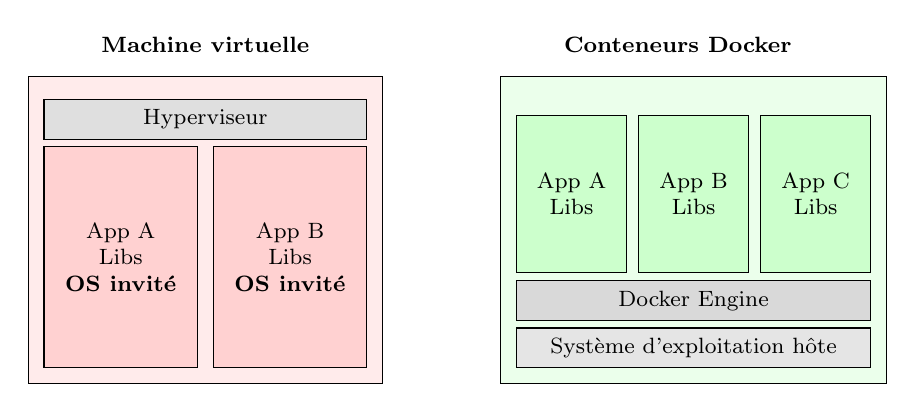
\begin{tikzpicture}[font=\footnotesize]
	% VM
	\node at (2.25,4.3) {\textbf{Machine virtuelle}};
	\draw[fill=red!8] (0,0) rectangle (4.5,3.9);
	\draw[fill=red!18] (0.2,0.2) rectangle (2.15,3.0) node[midway, align=center]{App A\\Libs\\\textbf{OS invité}};
	\draw[fill=red!18] (2.35,0.2) rectangle (4.3,3.0) node[midway, align=center]{App B\\Libs\\\textbf{OS invité}};
	\draw[fill=gray!25] (0.2,3.1) rectangle (4.3,3.6) node[midway]{Hyperviseur};
	% Conteneurs
	\node at (8.25,4.3) {\textbf{Conteneurs Docker}};
	\draw[fill=green!8] (6,0) rectangle (10.9,3.9);
	\draw[fill=green!20] (6.2,1.4) rectangle (7.6,3.4) node[midway, align=center]{App A\\Libs};
	\draw[fill=green!20] (7.75,1.4) rectangle (9.15,3.4) node[midway, align=center]{App B\\Libs};
	\draw[fill=green!20] (9.3,1.4) rectangle (10.7,3.4) node[midway, align=center]{App C\\Libs};
	\draw[fill=gray!30] (6.2,0.8) rectangle (10.7,1.3) node[midway]{Docker Engine};
	\draw[fill=gray!20] (6.2,0.2) rectangle (10.7,0.7) node[midway]{Système d'exploitation hôte};
\end{tikzpicture}
\end{center}
\noindent\textit{Figure~: la VM virtualise tout un OS, le conteneur partage le noyau hôte (plus léger).}

\newpage

\subsubsection*{JWT (JSON Web Token)}
\phantomsection
\addcontentsline{toc}{subsection}{JWT (JSON Web Token)}

\noindent Le \textbf{JWT} (\textit{JSON Web Token}, norme \textbf{RFC 7519}) est un standard ouvert définissant un format \textbf{compact et autoportant} pour échanger de manière sécurisée des informations sous forme d'objet \textbf{JSON}. Un JWT se compose de \textbf{trois parties} encodées en Base64URL et séparées par des points~:
\begin{itemize}
	\item \textbf{En-tête} (\textit{header})~: l'\textbf{algorithme} de signature (ex.~\texttt{HS256}) et le type de jeton.
	\item \textbf{Charge utile} (\textit{payload})~: les \textbf{revendications} (\textit{claims}) — identité de l'utilisateur, rôle, date d'expiration (\texttt{exp})…
	\item \textbf{Signature}~: garantit l'\textbf{intégrité} et l'\textbf{authenticité} du jeton.
\end{itemize}
\begin{center}
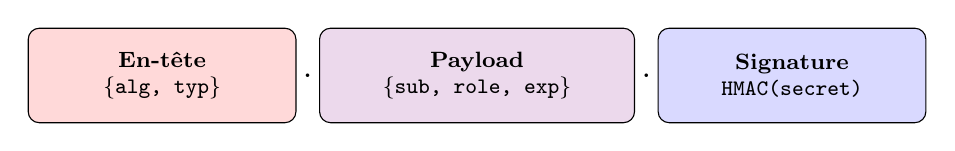
\begin{tikzpicture}[font=\footnotesize]
	\draw[fill=red!15, rounded corners] (0,0) rectangle (3.4,1.2) node[midway, align=center]{\textbf{En-tête}\\\texttt{\{alg, typ\}}};
	\draw[fill=violet!15, rounded corners] (3.7,0) rectangle (7.7,1.2) node[midway, align=center]{\textbf{Payload}\\\texttt{\{sub, role, exp\}}};
	\draw[fill=blue!15, rounded corners] (8.0,0) rectangle (11.4,1.2) node[midway, align=center]{\textbf{Signature}\\\texttt{HMAC(secret)}};
	\node at (3.55,0.6) {\textbf{.}};
	\node at (7.85,0.6) {\textbf{.}};
\end{tikzpicture}
\end{center}
\noindent\textit{Figure~: les trois parties d'un JWT — \texttt{xxxxx.yyyyy.zzzzz}.}

\noindent Sa signature cryptographique permet au serveur de \textbf{vérifier la validité} du jeton \textbf{sans conserver d'état de session} (\textit{stateless})~: idéal pour des micro-services indépendants. Exemple de \textit{payload}~:
\begin{minted}[fontsize=\footnotesize, bgcolor=gray!8]{json}
{ "sub": "user_42", "name": "Yanis", "role": "admin", "exp": 1735689600 }
\end{minted}

\vspace{0.4cm}

\subsubsection*{Jetons / Tokens}
\phantomsection
\addcontentsline{toc}{subsection}{Jetons / Tokens}

\noindent Un \textbf{jeton} (ou \textit{token}) est une donnée numérique délivrée par un serveur d'authentification qui \textbf{matérialise et atteste des droits} d'un utilisateur au sein d'un système. Il remplace l'envoi répété des identifiants~: une fois authentifié, l'utilisateur reçoit un jeton qu'il \textbf{joint à chacune de ses requêtes} (en-tête HTTP \texttt{Authorization: Bearer <token>}) pour prouver son identité. On distingue~:
\begin{itemize}
	\item l'\textbf{\textit{access token}} (jeton d'accès)~: \textbf{courte durée de vie}, présenté à chaque requête pour accéder aux ressources~;
	\item le \textbf{\textit{refresh token}} (jeton de rafraîchissement)~: \textbf{longue durée de vie}, qui permet d'obtenir un nouvel \textit{access token} \textbf{sans se reconnecter}.
\end{itemize}
\noindent Dans le projet, ces jetons sont des \textbf{JWT}~: c'est le mécanisme retenu pour sécuriser les échanges entre le front-end et les micro-services.

\newpage

\subsubsection*{Authentification}
\phantomsection
\addcontentsline{toc}{subsection}{Authentification}

\noindent L'\textbf{authentification} (\textit{AuthN}) est le processus qui consiste à \textbf{vérifier l'identité} d'un utilisateur avant de lui accorder l'accès. Elle répond à la question «~\textbf{Qui êtes-vous~?}~» en confrontant une \textbf{preuve} (mot de passe, jeton, certificat, biométrie) à une référence connue du système. Elle se distingue de l'\textbf{autorisation} (\og{}qu'avez-vous le droit de faire~?\fg{}), qui intervient \textbf{ensuite}. Dans une architecture à jetons, l'authentification aboutit à la \textbf{délivrance d'un JWT}~:
\begin{center}
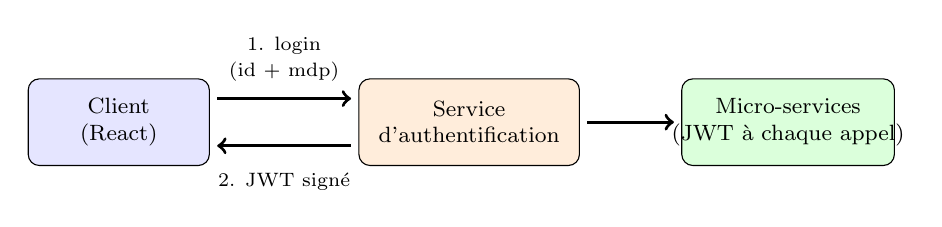
\begin{tikzpicture}[font=\footnotesize]
	\draw[fill=blue!10, rounded corners] (0,0.6) rectangle (2.3,1.7) node[midway, align=center]{Client\\(React)};
	\draw[fill=orange!14, rounded corners] (4.2,0.6) rectangle (7.0,1.7) node[midway, align=center]{Service\\d'authentification};
	\draw[->, very thick] (2.4,1.45) -- (4.1,1.45); \node[align=center] at (3.25,1.95){\scriptsize 1. login\\\scriptsize (id + mdp)};
	\draw[<-, very thick] (2.4,0.85) -- (4.1,0.85); \node[align=center] at (3.25,0.4){\scriptsize 2. JWT signé};
	\draw[->, very thick] (7.1,1.15) .. controls (8.2,1.15) .. (8.2,1.15);
	\draw[fill=green!14, rounded corners] (8.3,0.6) rectangle (11.0,1.7) node[midway, align=center]{Micro-services\\(JWT à chaque appel)};
\end{tikzpicture}
\end{center}
\noindent\textit{Figure~: l'utilisateur s'authentifie une fois, reçoit un JWT, puis le présente à chaque micro-service.} L'authentification peut être renforcée par \textbf{plusieurs facteurs} (\textbf{MFA}). C'est l'objet de l'AAV \og{}Réaliser un système d'authentification dans une API\fg{}.

\vspace{0.4cm}

\subsubsection*{API Gateway}
\phantomsection
\addcontentsline{toc}{subsection}{API Gateway}

\noindent Une \textbf{API Gateway} (passerelle d'API) est le \textbf{point d'entrée unique} d'une architecture micro-services. Tous les appels clients passent par elle, et elle se charge de les \textbf{router} vers le bon service. Elle centralise des préoccupations transverses qu'il serait coûteux de dupliquer dans chaque service~:
\begin{itemize}
	\item \textbf{routage} et agrégation des requêtes~;
	\item \textbf{authentification / autorisation}~: \textbf{validation des jetons JWT} en amont des services~;
	\item \textbf{limitation de débit} (\textit{rate limiting}), journalisation, mise en cache~;
	\item \textbf{terminaison TLS} et masquage de la structure interne.
\end{itemize}
\begin{center}
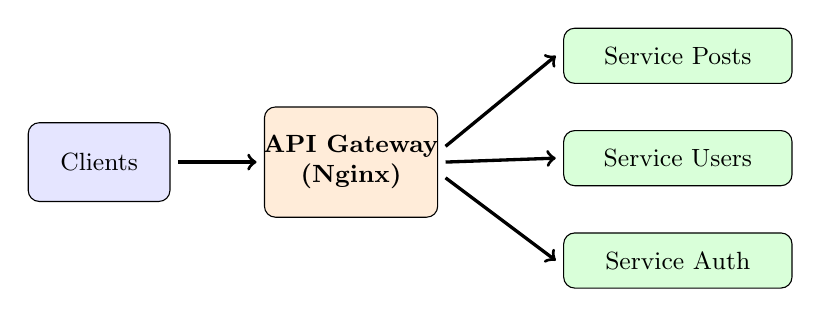
\begin{tikzpicture}[font=\small]
	\draw[fill=blue!10, rounded corners] (0,0.8) rectangle (1.8,1.8) node[midway]{Clients};
	\draw[fill=orange!15, rounded corners] (3,0.6) rectangle (5.2,2.0) node[midway, align=center]{\textbf{API Gateway}\\\textbf{(Nginx)}};
	\draw[->, very thick] (1.9,1.3) -- (2.9,1.3);
	\draw[fill=green!15, rounded corners] (6.8,2.3) rectangle (9.7,3.0) node[midway]{Service Posts};
	\draw[fill=green!15, rounded corners] (6.8,1.0) rectangle (9.7,1.7) node[midway]{Service Users};
	\draw[fill=green!15, rounded corners] (6.8,-0.3) rectangle (9.7,0.4) node[midway]{Service Auth};
	\draw[->, very thick] (5.3,1.5) -- (6.7,2.65);
	\draw[->, very thick] (5.3,1.3) -- (6.7,1.35);
	\draw[->, very thick] (5.3,1.1) -- (6.7,0.05);
\end{tikzpicture}
\end{center}
\noindent\textit{Figure~: l'API Gateway (Nginx) route les requêtes et valide les JWT avant d'atteindre les micro-services.}

\newpage

\subsubsection*{Micro-services}
\phantomsection
\addcontentsline{toc}{subsection}{Micro-services}

\noindent L'\textbf{architecture en micro-services} (MSA) consiste à découper une application en un ensemble de \textbf{petits services autonomes}, chacun responsable d'une seule capacité métier (posts, utilisateurs, authentification…). Chaque service~:
\begin{itemize}
	\item est \textbf{développé, déployé et mis à l'échelle indépendamment} des autres~;
	\item possède idéalement sa \textbf{propre base de données} (\textit{Database per Service})~;
	\item communique via des \textbf{interfaces réseau légères}, le plus souvent des \textbf{API REST} en HTTP/JSON.
\end{itemize}
\noindent \textbf{Avantages}~: scalabilité fine, résilience (une panne reste isolée), déploiements indépendants. \textbf{Inconvénients}~: complexité accrue (réseau, supervision) et nécessité d'une \textbf{API Gateway} ainsi que d'une stratégie de \textbf{sécurité distribuée} — ce qui justifie précisément le recours aux \textbf{jetons JWT} dans ce projet, chaque service vérifiant le jeton de façon autonome.

\vspace{0.4cm}

\subsubsection*{Multi-conteneurs}
\phantomsection
\addcontentsline{toc}{subsection}{Multi-conteneurs}

\noindent Une application \textbf{multi-conteneurs} est une application dont les différents composants (chaque micro-service, sa base de données, la passerelle) s'exécutent dans des \textbf{conteneurs distincts mais coordonnés}. Chaque composant a son propre environnement isolé tout en communiquant via un \textbf{réseau partagé}. L'orchestration est assurée par \textbf{Docker Compose} (développement / déploiements simples) ou par un \textbf{orchestrateur} comme \textbf{Kubernetes} (production à grande échelle). Un fichier \texttt{docker-compose.yml} déclare l'ensemble des services~:
\begin{minted}[fontsize=\footnotesize, bgcolor=gray!8]{yaml}
services:
  gateway:   { image: nginx, ports: ["80:80"] }      # passerelle
  auth:      { build: ./auth-service }               # délivre les JWT
  users:     { build: ./users-service }              # micro-service métier
  mongo:     { image: mongo }                         # base de données
\end{minted}
\noindent Une seule commande (\texttt{docker compose up}) démarre alors \textbf{toute la pile} de Yanis~: passerelle, service d'authentification, micro-services et base de données.

\vspace{0.4cm}

\newpage

\subsubsection*{Autorisation (Contrôle d'accès)}
\phantomsection
\addcontentsline{toc}{subsection}{Autorisation (Contrôle d'accès)}

\noindent L'\textbf{autorisation} (\textit{AuthZ}), ou \textbf{contrôle d'accès}, détermine les \textbf{ressources et actions} auxquelles un utilisateur \textbf{déjà authentifié} a le droit d'accéder. Elle répond à la question «~\textbf{Qu'avez-vous le droit de faire~?}~» et intervient \textbf{toujours après} l'authentification. Le modèle le plus courant est le \textbf{RBAC} (\textit{Role-Based Access Control})~: des \textbf{permissions} sont attribuées à des \textbf{rôles}, eux-mêmes assignés aux utilisateurs.

\begin{center}
\begin{tabular}{|l|l|l|}
\hline
\textbf{Rôle} & \textbf{Lire} & \textbf{Supprimer} \\ \hline
\texttt{visiteur} & oui & non \\ \hline
\texttt{membre}   & oui & ses propres posts \\ \hline
\texttt{admin}    & oui & tous les posts \\ \hline
\end{tabular}
\end{center}

\noindent Dans une architecture à jetons, le \textbf{rôle} de l'utilisateur est encodé dans les \textbf{revendications (\textit{claims})} du \textbf{JWT} et \textbf{vérifié à chaque requête} par le micro-service concerné. C'est la réponse aux AAV \og{}Mettre en place le contrôle d'accès dans une application backend\fg{} et \og{}Proposer un contrôle d'accès pour une application front\fg{}.

\section*{Analyse et résolution : JWT Docker}
\addcontentsline{toc}{section}{Analyse et résolution : JWT Docker}

\noindent \textit{Rappel de la problématique~:} \og{}Comment sécuriser l'accès aux micro-services d'une application web MERN, en utilisant des jetons JWT pour l'authentification et le contrôle d'accès, tout en automatisant le déploiement de ces services avec Docker~?\fg{}

\vspace{0.3cm}

\noindent La réponse se construit en six étapes~: \textbf{(1)} le choix du \textbf{mécanisme d'authentification} par jeton (service maison \textit{vs} service tiers), \textbf{(2)} l'\textbf{architecture cible} (service d'authentification indépendant derrière une API Gateway), \textbf{(3)} la \textbf{génération et la validation des JWT} dans l'API, \textbf{(4)} le \textbf{contrôle d'accès back-end}, \textbf{(5)} le \textbf{contrôle d'accès front-end}, et \textbf{(6)} la \textbf{conteneurisation Docker} et l'automatisation du déploiement. Une synthèse argumentée clôt l'analyse.

\vspace{0.4cm}

\subsection*{1. Mécanisme d'authentification~: pourquoi des jetons JWT}
\phantomsection
\addcontentsline{toc}{subsection}{1. Mécanisme d'authentification (JWT)}
\noindent Dans une architecture \textbf{micro-services}, l'authentification par \textbf{session serveur} est mal adaptée~: elle suppose un état partagé entre des services censés rester \textbf{indépendants et sans état}. La solution retenue est l'authentification par \textbf{jeton JWT}~: après connexion, l'utilisateur reçoit un jeton \textbf{signé} qu'il présente à chaque requête, et que \textbf{chaque service vérifie seul} grâce à la signature, sans interroger une base de sessions centrale.

\noindent Deux approches sont possibles pour \textbf{émettre} ces jetons~:
\begin{itemize}
	\item \textbf{Service maison}~: un micro-service d'authentification développé en Node.js (bibliothèque \texttt{jsonwebtoken}) qui signe et vérifie les JWT. Simple, totalement maîtrisé, suffisant pour le périmètre du projet.
	\item \textbf{Service tiers d'identité} (\textbf{Auth0}, \textbf{Keycloak})~: un fournisseur externe qui délègue l'authentification via les protocoles standard \textbf{OAuth~2.0 / OpenID Connect}. L'application ne gère plus les mots de passe~; elle reçoit un JWT émis par le tiers. Avantages~: \textbf{SSO}, MFA, gestion des comptes externalisée et conformité.
\end{itemize}
\noindent \textbf{Décision}~: un \textbf{service d'authentification dédié} est créé (réponse à l'AAV \og{}Réaliser un système d'authentification dans une API\fg{}), l'architecture restant \textbf{compatible} avec un futur basculement vers un \textbf{service tiers} (Keycloak), puisque dans les deux cas les services consommateurs ne font que \textbf{valider un JWT}.

\vspace{0.4cm}

\subsection*{2. Architecture cible~: service d'authentification + API Gateway}
\phantomsection
\addcontentsline{toc}{subsection}{2. Architecture cible}
\noindent La nouvelle architecture isole l'authentification dans un \textbf{micro-service indépendant} et place une \textbf{API Gateway (Nginx)} en \textbf{point d'entrée unique}. Le parcours d'une requête est le suivant~:
\begin{enumerate}
	\item le client s'authentifie auprès du \textbf{service d'authentification} et obtient un \textbf{JWT}~;
	\item il joint ce jeton (\texttt{Authorization: Bearer <token>}) à chacun de ses appels~;
	\item la \textbf{Gateway} reçoit la requête, \textbf{valide le JWT}, puis la \textbf{route} vers le micro-service métier visé~;
	\item le micro-service, qui reçoit une requête déjà authentifiée, applique le \textbf{contrôle d'accès} selon le rôle.
\end{enumerate}
\noindent Cette séparation respecte le principe \textbf{une responsabilité par service} et centralise la sécurité au bon endroit (la Gateway pour la \textbf{validation}, chaque service pour l'\textbf{autorisation} métier).

\vspace{0.4cm}

\subsection*{3. Génération et validation des JWT dans l'API}
\phantomsection
\addcontentsline{toc}{subsection}{3. Génération et validation des JWT}
\noindent Le service d'authentification expose une route de \textbf{connexion} qui vérifie les identifiants, puis \textbf{signe un JWT} contenant les \textit{claims} utiles (identifiant et rôle), avec une \textbf{courte durée de vie}~:

\begin{minted}[fontsize=\footnotesize, bgcolor=gray!8]{javascript}
const jwt = require('jsonwebtoken');
const SECRET = process.env.JWT_SECRET;            // secret en variable d'env.

// POST /api/auth/login  ->  authentifie puis délivre un JWT
async function login(req, res) {
  const user = await User.findOne({ email: req.body.email });
  const ok = user && await bcrypt.compare(req.body.password, user.hash);
  if (!ok) return res.status(401).json({ erreur: 'Identifiants invalides' });

  const token = jwt.sign(
    { sub: user.id, role: user.role },            // claims (identité + rôle)
    SECRET,
    { expiresIn: '15m' }                          // jeton à courte durée de vie
  );
  res.json({ token });
}
\end{minted}

\noindent Côté micro-services, un \textbf{middleware} extrait le jeton de l'en-tête \texttt{Authorization} et le \textbf{vérifie} (signature + expiration). En cas d'échec, l'accès est refusé (\texttt{401})~:

\begin{minted}[fontsize=\footnotesize, bgcolor=gray!8]{javascript}
// Middleware : vérifie le JWT présent dans l'en-tête Authorization
function authentifier(req, res, next) {
  const header = req.headers.authorization || '';
  const token  = header.startsWith('Bearer ') ? header.slice(7) : null;
  if (!token) return res.status(401).json({ erreur: 'Jeton manquant' });
  try {
    req.utilisateur = jwt.verify(token, SECRET);  // payload vérifié et décodé
    next();
  } catch {
    res.status(401).json({ erreur: 'Jeton invalide ou expiré' });
  }
}
\end{minted}

\noindent C'est la réponse aux AAV \og{}Réaliser un système d'authentification dans une API\fg{} et \og{}Gérer la sécurité de l'application à l'aide de jetons\fg{}~: le jeton, \textbf{signé et daté}, est validé de manière \textbf{autonome} par chaque service.

\newpage

\subsection*{4. Contrôle d'accès côté back-end (RBAC)}
\phantomsection
\addcontentsline{toc}{subsection}{4. Contrôle d'accès back-end}
\noindent Une fois l'utilisateur \textbf{authentifié}, le service applique l'\textbf{autorisation} en lisant le \textbf{rôle} contenu dans les \textit{claims} du JWT. Un second middleware, paramétré par les rôles autorisés, implémente le \textbf{RBAC}~:

\begin{minted}[fontsize=\footnotesize, bgcolor=gray!8]{javascript}
// Contrôle d'accès basé sur les rôles (RBAC)
function autoriser(...roles) {
  return (req, res, next) => {
    if (!roles.includes(req.utilisateur.role))
      return res.status(403).json({ erreur: 'Accès interdit' });   // 403
    next();
  };
}

// Exemple : seul un admin peut supprimer un post
router.delete('/api/posts/:id', authentifier, autoriser('admin'), supprimerPost);
\end{minted}

\noindent La chaîne \texttt{authentifier → autoriser → contrôleur} sépare clairement les deux responsabilités~: \textbf{qui es-tu} (\texttt{401} si le jeton est invalide) puis \textbf{as-tu le droit} (\texttt{403} si le rôle est insuffisant). C'est la réponse à l'AAV \og{}Mettre en place le contrôle d'accès dans une application backend\fg{}.

\vspace{0.4cm}

\subsection*{5. Contrôle d'accès côté front-end}
\phantomsection
\addcontentsline{toc}{subsection}{5. Contrôle d'accès front-end}
\noindent Côté React, deux mécanismes sont mis en place. D'abord un \textbf{intercepteur Axios} qui \textbf{joint automatiquement le JWT} à chaque requête sortante~:

\begin{minted}[fontsize=\footnotesize, bgcolor=gray!8]{jsx}
// Intercepteur Axios : ajoute le JWT à chaque requête
api.interceptors.request.use((config) => {
  const token = localStorage.getItem('token');
  if (token) config.headers.Authorization = `Bearer ${token}`;
  return config;
});
\end{minted}

\noindent Ensuite des \textbf{routes protégées} qui masquent ou redirigent selon l'état d'authentification et le rôle~:

\begin{minted}[fontsize=\footnotesize, bgcolor=gray!8]{jsx}
// Route protégée : redirige si non authentifié ou rôle insuffisant
function RouteProtegee({ children, role }) {
  const user = useAuth();                          // décode le JWT stocké
  if (!user)                       return <Navigate to="/login" />;
  if (role && user.role !== role)  return <Navigate to="/403" />;
  return children;
}
\end{minted}

\noindent \textbf{Point de sécurité essentiel}~: le contrôle d'accès front-end relève uniquement de l'\textbf{expérience utilisateur} (ne pas afficher de boutons inutiles, rediriger proprement). Il est \textbf{contournable} et ne constitue \textbf{jamais} une protection~: la sécurité réelle est \textbf{toujours imposée côté back-end}. C'est la réponse à l'AAV \og{}Proposer un contrôle d'accès pour une application front\fg{}.

\newpage

\subsection*{6. Conteneurisation Docker et automatisation du déploiement}
\phantomsection
\addcontentsline{toc}{subsection}{6. Conteneurisation et déploiement}
\noindent Chaque brique (service d'authentification, micro-services, Gateway, base) est \textbf{conteneurisée} via un \texttt{Dockerfile} dédié, garantissant une exécution \textbf{identique} du poste de Yanis à la production~:

\begin{minted}[fontsize=\footnotesize, bgcolor=gray!8]{docker}
FROM node:20-alpine            # image légère
WORKDIR /app
COPY package*.json ./
RUN npm ci --omit=dev          # dépendances de production uniquement
COPY . .
EXPOSE 4000
CMD ["node", "server.js"]      # point d'entrée du service
\end{minted}

\noindent La \textbf{Gateway Nginx} route le trafic et \textbf{délègue la validation du jeton} au service d'authentification (sous-requête \texttt{auth\_request}) avant de transmettre aux services métier~:

\begin{minted}[fontsize=\footnotesize, bgcolor=gray!8]{nginx}
upstream auth  { server auth:4000; }
upstream users { server users:5000; }

server {
  listen 80;
  location /api/auth/  { proxy_pass http://auth; }   # login / refresh (public)
  location /api/users/ {
    auth_request /verify;                            # valide le JWT en amont
    proxy_pass http://users;
  }
  location = /verify { internal; proxy_pass http://auth/verify; }
}
\end{minted}

\noindent Enfin, l'ensemble est orchestré en \textbf{multi-conteneurs} par \textbf{Docker Compose} (cf.~\texttt{docker-compose.yml} en partie \og{}Mots clés\fg{})~: une seule commande \texttt{docker compose up} démarre toute la pile. Pour la \textbf{production à grande échelle}, ce même socle conteneurisé se déploie sur un \textbf{orchestrateur} (\textbf{Kubernetes / AWS EKS}), qui apporte \textbf{scalabilité}, \textbf{auto-réparation} et déploiements progressifs sans interruption — répondant à l'objectif d'\textbf{automatisation du déploiement}.

\vspace{0.4cm}

\subsection*{7. Architecture retenue (schéma argumenté)}
\phantomsection
\addcontentsline{toc}{subsection}{7. Architecture retenue}
\noindent L'architecture cible combine tous ces éléments~: le client React obtient un JWT auprès du \textbf{service d'authentification}, puis tous ses appels transitent par la \textbf{Gateway Nginx} qui \textbf{valide le jeton} et \textbf{route} vers des \textbf{micro-services conteneurisés}, chacun appliquant son \textbf{contrôle d'accès} et disposant de sa \textbf{propre base MongoDB}, le tout déployé en \textbf{conteneurs Docker}.
\begin{center}
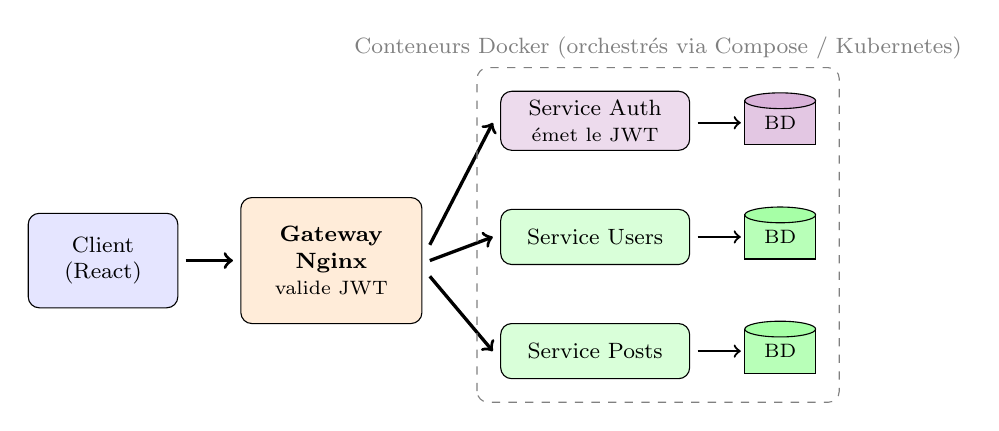
\begin{tikzpicture}[font=\footnotesize]
	\draw[fill=blue!10, rounded corners] (0,1.3) rectangle (1.9,2.5) node[midway, align=center]{Client\\(React)};
	\draw[fill=orange!15, rounded corners] (2.7,1.1) rectangle (5.0,2.7) node[midway, align=center]{\textbf{Gateway}\\\textbf{Nginx}\\\scriptsize valide JWT};
	\draw[->, very thick] (2.0,1.9) -- (2.6,1.9);
	% service auth
	\draw[fill=violet!14, rounded corners] (6.0,3.3) rectangle (8.4,4.05) node[midway, align=center]{Service Auth\\\scriptsize émet le JWT};
	% micro-services
	\draw[fill=green!15, rounded corners] (6.0,1.85) rectangle (8.4,2.55) node[midway]{Service Users};
	\draw[fill=green!15, rounded corners] (6.0,0.4) rectangle (8.4,1.1) node[midway]{Service Posts};
	\draw[->, very thick] (5.1,2.1) -- (5.9,3.65);
	\draw[->, very thick] (5.1,1.9) -- (5.9,2.2);
	\draw[->, very thick] (5.1,1.7) -- (5.9,0.75);
	% bases
	\foreach \y in {2.2,0.75} {
		\draw[fill=green!28] (9.1,\y-0.28) rectangle (10.0,\y+0.28);
		\draw[fill=green!35] (9.55,\y+0.28) ellipse (0.45 and 0.1);
		\node at (9.55,\y) {\scriptsize BD};
		\draw[->, thick] (8.5,\y) -- (9.05,\y);
	}
	\draw[fill=violet!22] (9.1,3.65-0.28) rectangle (10.0,3.65+0.28);
	\draw[fill=violet!30] (9.55,3.65+0.28) ellipse (0.45 and 0.1);
	\node at (9.55,3.65) {\scriptsize BD};
	\draw[->, thick] (8.5,3.65) -- (9.05,3.65);
	% englobant Docker
	\draw[dashed, gray, rounded corners] (5.7,0.1) rectangle (10.3,4.35);
	\node[gray] at (8.0,4.6) {\footnotesize Conteneurs Docker (orchestrés via Compose / Kubernetes)};
\end{tikzpicture}
\end{center}
\noindent\textit{Figure~: architecture retenue — service d'authentification émettant les JWT, Gateway Nginx validant et routant, micro-services conteneurisés avec base par service.}

\vspace{0.2cm}

\noindent \textbf{Justification}~: chaque exigence de la problématique est satisfaite — \textbf{authentification} par un service dédié, \textbf{sécurité par jetons JWT} signés et validés sans état, \textbf{contrôle d'accès} RBAC back-end (et UX front-end), point d'entrée unique \textbf{Gateway Nginx}, et \textbf{déploiement automatisé} grâce à Docker et à l'orchestration.

\newpage

\subsection*{Conclusion}
\phantomsection
\addcontentsline{toc}{subsection}{Conclusion}
\noindent \textbf{En réponse à la problématique}, sécuriser l'accès aux micro-services d'une application MERN ne tient pas à une mesure isolée mais à une \textbf{chaîne de décisions cohérentes}. L'authentification est confiée à un \textbf{service dédié} qui délivre des \textbf{JWT} signés et à courte durée de vie~; ce choix \textit{stateless} est parfaitement adapté aux micro-services, qui \textbf{valident chacun le jeton de façon autonome} sans état partagé, tout en laissant la porte ouverte à un \textbf{service tiers} (Keycloak) si le besoin grandit.

\vspace{0.2cm}

\noindent La \textbf{sécurité par jetons} se décline ensuite en deux temps~: l'\textbf{authentification} (\texttt{401} si le jeton est absent ou invalide) puis l'\textbf{autorisation} \textbf{RBAC} fondée sur le rôle inscrit dans les \textit{claims} (\texttt{403} si le rôle est insuffisant). Côté front-end, les routes protégées et l'intercepteur Axios améliorent l'expérience, mais la \textbf{protection réelle reste imposée côté back-end}. Une \textbf{API Gateway Nginx} centralise la validation des jetons et le routage en point d'entrée unique.

\vspace{0.2cm}

\noindent Enfin, la \textbf{conteneurisation Docker} et l'orchestration \textbf{multi-conteneurs} (Docker Compose en développement, Kubernetes/EKS en production) \textbf{automatisent le déploiement} et assurent une exécution identique de bout en bout. L'ensemble constitue un \textbf{modèle reproductible}~: la démarche validée ici pourra être étendue, service après service, à toute l'application de l'entreprise.

\newpage

\section*{Capitalisation}
\addcontentsline{toc}{section}{Capitalisation}

\begin{center}
\setlength{\tabcolsep}{10pt}

\begin{tabular}{|p{0.30\textwidth}|p{0.45\textwidth}|m{0.08\textwidth}|}
\hline
\textbf{AAV} & \textbf{Commentaire} & \textbf{Statut} \\ \hline

Expliquer le fonctionnement d'un service tiers d'authentification &
Service maison (\texttt{jsonwebtoken}) comparé à un service tiers (Auth0/Keycloak, OAuth~2.0/OIDC)~: rôle du serveur d'autorisation et émission déléguée du JWT. &
{\color{green!60!black}Acquis} \\ \hline

Gérer la sécurité de l'application à l'aide de jetons &
JWT signés à courte durée de vie (+ \textit{refresh}), transmis en \texttt{Bearer} et validés sans état par chaque micro-service~; structure en-tête/payload/signature détaillée. &
{\color{green!60!black}Acquis} \\ \hline

Mettre en place le contrôle d'accès dans une application backend &
Middleware RBAC vérifiant le rôle inscrit dans les \textit{claims} du JWT (chaîne \texttt{authentifier → autoriser}, \texttt{401}/\texttt{403}), illustré par du code Express. &
{\color{green!60!black}Acquis} \\ \hline

Proposer un contrôle d'accès pour une application front &
Routes protégées React et intercepteur Axios joignant le JWT~; rappel que le contrôle front est UX et que la protection réelle reste côté back-end. &
{\color{green!60!black}Acquis} \\ \hline

Réaliser un système d'authentification dans une API &
Service d'authentification Express délivrant les JWT (route \texttt{login}, signature, expiration) et middleware de validation, illustrés par du code commenté. &
{\color{green!60!black}Acquis} \\ \hline

\end{tabular}
\end{center}

\newpage

\section*{Ressources}
\addcontentsline{toc}{section}{Ressources}

\begin{itemize}
	\item \textbf{JWT (introduction \& débogueur)} : \url{https://jwt.io/introduction}
	\item \textbf{RFC 7519 -- JSON Web Token} : \url{https://datatracker.ietf.org/doc/html/rfc7519}
	\item \textbf{Bibliothèque jsonwebtoken (Node.js)} : \url{https://github.com/auth0/node-jsonwebtoken}
	\item \textbf{Keycloak (service d'identité)} : \url{https://www.keycloak.org/documentation}
	\item \textbf{OAuth~2.0 / OpenID Connect} : \url{https://openid.net/developers/how-connect-works/}
	\item \textbf{Nginx -- module auth\_request} : \url{https://nginx.org/en/docs/http/ngx_http_auth_request_module.html}
	\item \textbf{Documentation Docker \& Compose} : \url{https://docs.docker.com/}
	\item \textbf{Amazon EKS (Kubernetes managé)} : \url{https://docs.aws.amazon.com/eks/}
	\item \textbf{OWASP -- bonnes pratiques d'authentification} : \url{https://cheatsheetseries.owasp.org/cheatsheets/Authentication_Cheat_Sheet.html}
\end{itemize}
